\documentclass[a4paper,12pt]{article}

\usepackage[utf8]{inputenc}
\usepackage{polski} %polski
\usepackage{graphics} %obrazki
\usepackage{hyperref} % linki
\usepackage{url} % wyświetlanie linków
\usepackage{float} %dodaje wymuszanie obrazków(H)
\usepackage[defaultlines=4,all]{nowidow} % zapobieganie wdowom
\usepackage[]{amsmath} % ładne wzorki
\usepackage{chemfig} % wzory chemiczne (strukturalne)

\begin{document}

\section{Wprowadzenie}

Związki nasycone: alkany, cykloalkany

Związki nienasycone: alkany, alkiny, aromatyczne, cykloalkeny, enyny
\newline

Enyny- zawierają wiązanie podwójne i potrójne [numerację zaczynamy od bliższego bądź gdy są w tej samej odległości to od podwójnego].
\newline

Węglowodory alifatyczne- wszystkie związki organiczne niearomatyczne (również te o łańcuchach zamkniętych).
\newline

\begin{figure}[H]
    \centering
    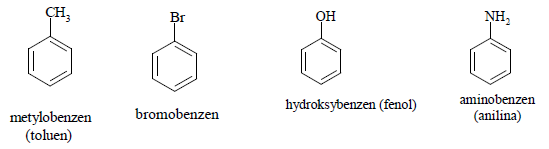
\includegraphics[width=0.7\textwidth]{img/benzeny}
    \label{fig.benzeny}
\end{figure}

\begin{figure}[H]
    \centering
    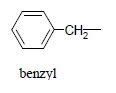
\includegraphics[width=0.2\textwidth]{img/benzyl}
    \label{fig.benzyl}
\end{figure}

\begin{figure}[H]
    \centering
    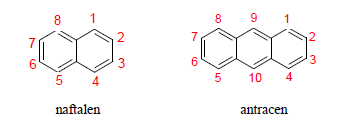
\includegraphics[width=0.7\textwidth]{img/naftalen}
    \label{fig.naftalen}
\end{figure}

\section{Grupy funkcyjne}
\begin{itemize}
    \item Alkohole
    
    \chemfig[atom sep=2em]{R-OH}
    \newline

    Nazwę związku tworzy się na dwa sposoby. Możemy napisać  "alkohol..." w miejscu kropek wstawiając nazwę związku (łańcucha). Drugim sposobem jest do nazwy łańcucha dodać końcówkę -ol (-3-ol w momencie, gdy grupa hydroksylowa jest dołączona do trzeciego z kolei atomu węgla, itp.).

    \begin{center}
        Przykład:
        
        \chemfig[atom sep=2em]{CH_3-CH(-[6]OH)-CH_3}
        
        alkohol izopropylowy lub propan-2-ol
    \end{center}

    \item Etery
    
    \chemfig[atom sep=2em]{-C-O-C-}
    \newline

    Etery proste, nie zawierające żadnych innych grup funkcyjnych – po słowie eter wymienia się w kolejności alfabetycznej nazwy grup węglowodorowych połączonych z atomem tlenu. Można też etery proste nazywać podstawnikowo, w sposób opisany dla eterów złożonych. Etery symetryczne, w których z atomem tlenu połączone są takie same grupy węglowodorowe, nazywa się podając po słowie eter nazwę grupy węglowodorowej z przedrostkiem –di.

    Etery o bardziej złożonej budowie – nazwę tworzy się jako pochodną macierzystego węglowodoru i dodaje nazwę grupy węglowodorowej przyłączonej do atomu tlenu z końcówką –oksy. Grupę węglowodorową związaną z atomem tlenu traktuje się więc w tym przypadku jak podstawnik w cząsteczce węglowodoru stanowiącego podstawę nazwy.
    \newline

    \begin{center}
    Przykład:

    \chemfig[atom sep=2em]{CH_3-O-CH_2-CH_2-CH_3}
    
    eter metylowo-propylowy lub metoksypropan
\end{center}
    \item Aldehydy
    
    \chemfig[atom sep=2em]{-CHO}

    Nazwę aldehydu tworzy się dodając do nazwy macierzystego alkanu przyrostek –al.

    Niektóre proste aldehydy mają nazwy zwyczajowe, np.: formaldehyd, benzaldehyd.

    \begin{figure}[H]
        \centering
        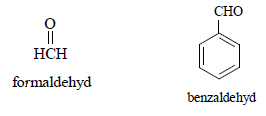
\includegraphics[width=0.5\textwidth]{img/formaldehyd}
        \label{fig.formaldehyd}
    \end{figure}

    \begin{center}
        Przykład:
    
        \chemfig[atom sep=2em]{CH_3-CH_2-CH=[2]O}
        
        propanal
    \end{center}

    \item Ketony
    
    \chemfig[atom sep=2em]{-C=O}

    Nazwę ketonu tworzy się od nazwy macierzystego alkanu dodając przyrostek –on, poprzedzony numerem atomu węgla z grupą karbonylową.

    W przypadku niektórych prostszych związków z tej grupy nazwy tworzy się wymieniając w kolejności alfabetycznej nazwy grup połączonych z grupą karbonylową, poprzedzając je słowem „keton”.

    \begin{figure}[H]
        \centering
        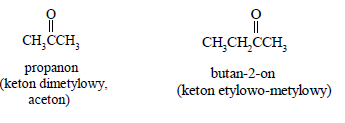
\includegraphics[width=0.7\textwidth]{img/keton}
        \label{fig.keton}
    \end{figure}
    \newpage
    \item Kwasy karboksylowe
    
    \chemfig[atom sep=2em]{-COOH}
    \newline

    Nazwy systematyczne kwasów karboksylowych tworzy się dwojako:
    \begin{enumerate}
        \item Do nazwy macierzystego alkanu z końcówką –owy dodaje się słowo kwas, a atom węgla w grupie karboksylowej jest oznaczany jako C1.
        \item Nazwa łańcucha głównego nie obejmuje grupy karboksylowej, a atom węgla, z którym połączona jest grupa karboksylowa, jest oznaczany jako C1. Do nazwy macierzystego alkanu dodaje się wówczas słowo kwas i końcówkę -karboksylowy.
    \end{enumerate}

    Niektóre związki można też nazwać zwyczajowo:

    \begin{figure}[H]
        \centering
        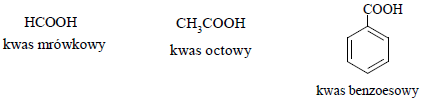
\includegraphics[width=0.7\textwidth]{img/mrówkowy}
        \label{fig.mrówkowy}
    \end{figure}

    \begin{center}
        Przykład:
    
        \chemfig[atom sep=2em]{CH_3-CH_2-COOH}
        
        kwas propanowy lub kwas etanokarboksylowy
    \end{center}

    \item Halogenki kwasowe
    
    \chemfig[atom sep=2em]{R-C(=[2]O)-X}

    Nazwy halogenków kwasowych tworzy się podając nazwę odpowiedniego halogenku i grupy acylowej (systematyczną lub zwyczajową). 

    \begin{center}
        Przykład:
    
        \chemfig[atom sep=2em]{CH_3-C(=[2]O)-Cl}
        
        Chlorek etanoilu

        Chlorek acetylu
    \end{center}

    Związki te można również nazywać w oparciu o nazwę kwasu macierzystego, poprzedzając ją nazwą odpowiedniego halogenku.

    \begin{center}
        Przykład:
    
        \chemfig[atom sep=2em]{CH_3-CH_2-C(=[2]O)-Br}
        
        Bromek kwasu propanowego
    \end{center}

    \item Bezwodniki kwasowy
    
    \chemfig[atom sep=2em]{R-C(=[2]O)-O-C(=[2]O)-R}

    W przypadku bezwodników symetrycznych (otrzymywanych z takiego samego kwasu karboksylowego) nazwy tworzy się, zastępując słowo kwas słowem bezwodnik lub dodając słowo bezwodnik do nazwy macierzystego kwasu.

    \begin{center}
        Przykład:
    
        \chemfig[atom sep=2em]{CH_3-C(=[2]O)-O-C(=[2]O)-CH_3}
        
        Bezwodnik octowy
    \end{center}

    Bezwodniki niesymetryczne (otrzymywane z różnych kwasów karboksylowych) nazywa się podobnie, przy czym nazwy kwasów podaje się w porządku alfabetycznym.

    \begin{center}
        Przykład:
    
        \chemfig[atom sep=2em]{CH_3-C(=[2]O)-O-C(=[2]O)-CH_2-CH_3}
        
        Bezwodnik octowo-propanowy
    \end{center}
    \newpage
    \item Estry
    
    \chemfig[atom sep=2em]{R-C(=[2]O)-O-R'}

    W nazwie estru określa się część kwasową i węglowodorową, najczęściej alkilową (wprowadzoną w miejsce atomu wodoru w grupie karboksylowej). Część kwasowa ma końcówkę –an lub –ian zamiast końcówki –owy występującej w nazwie kwasu macierzystego, część alkilowa (lub inna węglowodorowa) natomiast podawana jest w dopełniaczu.

    \begin{center}
        Przykład:
    
        \chemfig[atom sep=2em]{CH_3-CH_2-C(=[2]O)-O-CH_2-CH_3}
        
        Propanian etylu
    \end{center}

    W przypadku estrów kwasów łańcuchowych zawierających podstawniki w części kwasowej podaje się ich położenie w nazwie, oznaczając atom węgla grupy acylowej numerem 1. Gdy podstawniki znajdują się w części alkilowej (lub ogólnie: węglowodorowej)numeruje się atomy węgla tej części tak, że atom węgla łączący się z atomem tlenu ma numer 1.

    \begin{center}
        Przykład:
    
        \chemfig[atom sep=2em]{CH_3-C(-[2]CH_3)(-[6]CH_3)-CH_2-CH_2-C(=[6]O)-O-CH_3}
        
        4,4-dimetylopentanian metylu
    \end{center}

    \item Amidy
    
    \chemfig[atom sep=2em]{R-C(=[2]O)-NH_2}

    Nazwy amidów tworzy się, dodając do nazwy macierzystego alkanu końcówkę –oamid lub zamieniając końcówkę –yl (-oil) w nazwie grupy acylowej na przyrostek –amid.

    \begin{center}
        Przykłady:
    
        \chemfig[atom sep=2em]{CH_3-C(=[2]O)-NH_2}
        
        Acetamid
    \end{center}
    \begin{center}
         
        \chemfig[atom sep=2em]{CH_3-CH_2-CH_2-C(=[2]O)-NH_2}
        
        Butanoamid
    \end{center}

    Związki te można także określać, poprzedzając nazwę macierzystego kwasu karboksylowego słowem amid.

    \begin{center}
         Przykład:

        \chemfig[atom sep=2em]{CH_3-CH_2-C(=[2]O)-NH_2}
        
        Amid kwasu propanowego
    \end{center}

    W przypadku amidów podstawionych przy atomie azotu najpierw określa się podstawniki, a następnie podaje nazwę amidu macierzystego. Nazwę podstawników poprzedza się lokantem „N”, co oznacza bezpośrednie podstawienie przy atomie azotu.

    \begin{center}
        Przykład:

       \chemfig[atom sep=2em]{CH_3-CH(-[6]Br)-CH_2-C(=[2]O)-N(-[1]H)(-[7]CH_3)}
       
       N-metylo-3-bromobutanoamid
   \end{center}

    \item Nitrozwiązki
    
    \chemfig[atom sep=2em]{-NO_2}

    Do nazwy macierzystego węglowodoru dodaje się przedrostek nitro-. Grupę nitrową traktuje się jako podstawnik, a jej pozycję podaje się wymieniając numer atomu węgla, z którym jest ona związana.

    \begin{center}
        Przykład:

       \chemfig[atom sep=2em]{CH_3CH_2CH_2NO_2}
       
       1-nitropropan
   \end{center}
   \newpage
    \item Aminy
    \begin{enumerate}
        \item pierwszorzędowe
        
        \chemfig[atom sep=2em]{-NH_2}

        Nazwy tworzy się przez dodanie przyrostka –amina do nazwy podstawnika alkilowego. Aminę można potraktować również jako pochodną węglowodoru, zwłaszcza w przypadku amin zawierających inne grupy funkcyjne. Wówczas grupę $-NH_2$ można wymienić jako podstawnik aminowy oraz określić jego pozycję w związku macierzystym.

        \begin{center}
            Przykład:
    
           \chemfig[atom sep=2em]{CH_3CH_2CH_2-CH(-[6]NH_2)-CH_3}
           
           2-aminopentan
       \end{center}

       \begin{center}
        
            \chemfig[atom sep=2em]{CH_3CH_2-CH(-[2]NH_2)-COOH}
       
            kwas 2-aminobutanowy
        \end{center}

        \begin{center}
        
            \chemfig[atom sep=2em]{CH_2CH_2NH_2}
       
            etyloamina
        \end{center}

        \item drugorzędowe
        
        \chemfig[atom sep=2em]{-NH-}

        W przypadku symetrycznych amin do nazwy dodaje się przedrostek di- lub tri-, np.: difenyloamina, trietyloamina.

        \begin{center}
        
            \chemfig[atom sep=2em]{NH(-[2]CH_2CH_3)(-[5]CH_3CH_2)}
       
            dietyloamina
        \end{center}

        Aminy niesymetryczne drugorzędowe i trzeciorzędowe nazywa się jako N-podstawione aminy pierwszorzędowe. Nazwę największej grupy alkilowej wybiera się za nazwę macierzystą, a pozostałe grupy traktuje jako N-podstawniki (dołączone do atomu azotu), wymieniając je w kolejności alfabetycznej.

        \begin{center}
        
            \chemfig[atom sep=2em]{CH_3CH_2CH_2NHCH_3}
       
            N-metylopropyloamina
        \end{center}
        \item trzeciorzędowe
        
        \chemfig[atom sep=2em]{-N(-[6])-}

        \begin{center}
        
            \chemfig[atom sep=2em]{N(-[2]CH_2CH_3)(-[5]CH_3CH_2)(-[7]CH_2CH_3)}
       
            trietyloamina
        \end{center}

        \begin{center}
        
            \chemfig[atom sep=2em]{N(-[3]CH_3CH_2)(-[5]CH_3)-CH_2CH_2CH_2CH_3}
       
            N-etylo-N-metylobutyloamina
        \end{center}
        \item aminy aromatyczne
        \newline

        Aminy aromatyczne traktuje się jako pochodne aniliny (aminobenzenu), a grupy zastępujące atomy wodoru w grupie $NH_2$ aniliny - jako N-podstawniki.

        \begin{figure}[H]
            \centering
            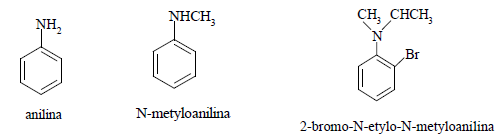
\includegraphics[width=0.7\textwidth]{img/anilina}
            \label{fig.anilina}
        \end{figure}
    \end{enumerate}
    

\end{itemize}


\section{Izomeria związków organicznych}

Izomeria- polega na zjawisku, że różne związki chemiczne mające ten sam wzór cząsteczkowy różnią się od siebie sposobem lub kolejnością wiązań chemicznych lub też rozmieszczeniem przestrzennym atomów.
\newline

Izomerię dzielimy na:
\begin{enumerate}
    \item konstytucyjną (strukturalną)- polega na występowaniu związków izomerycznych, w których atomy tych samych pierwiastków są ze sobą połączone w różnej kolejności.
    
    \begin{itemize}
        \item szkieletowa
        
        \begin{itemize}
            \item łańcuchowa- atomy węgla mogą przyjmować różne ułożenia w łańcuchu
            \item pierścieniowa
            \item łańcuchowo- pierścieniowa
        \end{itemize}
        \item podstawienia (położenia) 
        
        \begin{itemize}
            \item położenia podstawnika- różne położenie podstawników w cząsteczce
            \item położenia wiązania wielokrotnego- różne położenie wiązań nienasyconych (wielokrotnych)
        \end{itemize}
        \item funkcyjna- różne podstawniki w cząsteczce (grupy funkcyjne)
    \end{itemize}
    \item stereoizomerię (przestrzenna)- to szczególny rodzaj izomerii, gdzie atomy połączone są między sobą w identycznej kolejności ale różnią się sposobem rozmieszczenia atomów w przestrzeni.
    
    \begin{itemize}
        \item konformacyjna- stereoizomery różniące się między sobą rozmieszczeniem atomów w przestrzeni. Różne konformacje powstają przez obrót poszczególnych części cząsteczki wokół wiązań pojedyńczych i geometrycznie nie przystają do siebie.
        
        \begin{figure}[H]
            \centering
            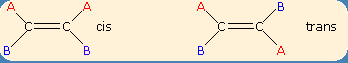
\includegraphics[width=0.7\textwidth]{img/izomer1}
            \label{fig.izomer1}
        \end{figure}
        \item geometryczna- Ten typ izomerii występuje wówczas, gdy w układzie przestrzennym cząsteczki zaznacza się określona płaszczyzna.
        Jeżeli wyróżnione grupy cząsteczki leżą po tej samej stronie płaszczyzny mamy do czynienia z izomerem cis a jeżeli po przeciwnych stronach z izomerem trans.

        \begin{figure}[H]
            \centering
            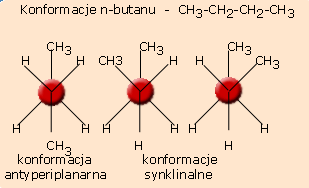
\includegraphics[width=0.7\textwidth]{img/izomery8}
            \label{fig.izomery8}
        \end{figure}
        \item optyczna- Jest to rodzaj stereoizomerii występującej w cząsteczkach chiralnych, które zawierają atom węgla, do którego przyłączone są cztery różne grupy. Taki atom nosi nazwę centrum chiralności.
        A to oznacza, że dla każdej cząsteczki posiadającej centrum chiralności możemy znalezć drugą cząsteczkę będącą jej lustrzanym odbiciem.

        Izomeria optyczna wiąże się ze zdolnością skręcania płaszczyzny światła spolaryzowanego. Substancje takie nazywa się optycznie czynnymi; skręcające płaszczyznę światła spolaryzowanego w prawo - nazywa się prawoskrętnymi /+/, a skręcajace w lewo -lewoskrętnymi /-/.

    \end{itemize}
\end{enumerate}

Izomeria optyczna:
\newline

Izomery bedące wzajemnymi odbiciami lustrzanymi noszą nazwę enacjomerów.

\newpage
Właściwości enancjomerów:
\begin{enumerate}
    \item Enancjomery mają identyczne właściwości fizyczne z wyjątkiem kierunku skręcania płaszczyzny polaryzacji światła
    \item Enancjomery wykazują identyczne właściwości chemiczne; wyjątkiem jest ich zachowanie się w stosunku do optycznie czynnych reagentów. Oznacza to, że jeżeli reagent jest optycznie czynny, jego wpływ na oba enancjomery nie jest identyczny podczas ataku i dlatego szybkość reakcji jest różna - w niektórych przypadkach tak dalece różna, że reakcja z jednym izomerem w ogóle nie zachodzi.
\end{enumerate}

Równocząsteczkowa mieszanina enacjomerów nie wykazuje optycznej czynności i nosi nazwę mieszaniny recemicznej.

Odmiana racemiczna jest optycznie nieczynna. Jest wynikiem równoważenia skręcalności cząsteczki jednego izomeru przez skręcalność cząsteczki drugiego izomeru.
W celu zaznaczenia racemicznego charakteru określonej próbki stosuje się znak (+/-), jak na przykład kwas (+/-)-mlekowy.
\newline

Konfiguracja D- i L-
\newline

Często dla względnego charakteryzowania cząstek chiralnych wprowadzono pojęcie konfiguracji D- i L-, co uwidocznione jest w nazwach związków. Na przykład - aldehyd D-glicerynowy, aldehyd L-glicerynowy

Punktem odniesienia dla konfiguracji D- i L- jest budowa cząsteczki aldehydu glicerynowego a konkretnie położenie podstawników H- oraz HO- przy środkowym węglu.

\begin{figure}[H]
    \centering
    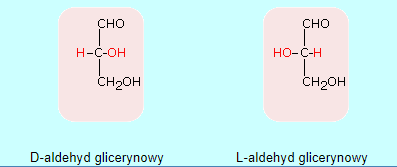
\includegraphics[width=0.7\textwidth]{img/D_L}
    \label{fig.D_L}
\end{figure}

Uporządkowanie na szeregi D i L następuje według konfiguracji podstawników, przy czym bierzemy pod uwagę to centrum chiralności, które jest najbardziej oddalone od grupy karbonylowej.

\section{Reakcje węglowodorów}

Wśród reakcji, którym ulegają węglowodory można wyróżnić cztery podstawowe typy: 

\begin{enumerate}
    \item substytucja- ulegają jej tylko węglowodory nasycone (alkany) i aromatyczne. Reakcja ta zachodzi pod wpływem naświetlania. Przykładem substytucji może być reakcja podstawienia jednego atomu wodoru przez atom chloru w cząsteczce metanu. W reakcji tej otrzymujemy chlorowcopochodną metanu i kwas solny. Reakcję taką przedstawia równanie:

    \schemestart
        \chemfig{CH_3}
        \+
        \chemfig{Cl_2}
        \arrow{->}
        \chemfig[atom sep=2em]{CH_3-Cl}
        \+
        \chemfig{HCl}
    \schemestop
    \item addycja- ulegają jej wyłącznie węglowodory aromatyczne i nienasycone. Addycja polega na rozerwaniu wiązania podwójnego i przyłączeniu się cząsteczki, która bierze udział w tej reakcji. Nie powstają żadne produkty uboczne. Do węglowodorów mogą się przyłączać:

    \begin{itemize}
        \item cząsteczki homoatomowe (zawierające dwa takie same atomy, np. Cl2, Br2 i H2)
        
        \schemestart
            \chemfig[atom sep=2em]{CH_2=CH-CH_3}
            \+
            \chemfig{H_2}
            \arrow{->}
            \chemfig[atom sep=2em]{CH_3-CH_2-CH_3}
        \schemestop

        Wiązanie podwójne między pierwszymi dwoma atomami węgla w cząsteczce propenu uległo rozerwaniu i przyłączyły się dwa atomy wodoru. Powstał propan.
        \item cząsteczki heteroatomowe (np. HCl, HI, HBr)
        
        W tym przypadku sytuacja jest bardzo podobna. Wiązanie podwójne ulega rozerwaniu, a atom wodoru przyłącza się do tego atomu węgla w cząsteczce węglowodoru, przy którym przed reakcją było więcej atomów wodoru (reguła Markownikowa). Gdy wodór się tak przyłączy powstanie wówczas produkt główny. Należy jednak pamiętać, że w reakcji tej powstanie także produkt uboczny, który będzie wynikiem podstawienie wodoru do atomu węgla, który przed reakcją zawierał mniejszą ilość atomów wodoru. Obydwa produkty powstaną równocześnie, jednak produktu głównego jest znacznie więcej.

        \schemestart
            \chemfig[atom sep=2em]{CH_3CH=CH_2}
            \+
            \chemfig{HBr}
            \arrow{->}
            \chemfig[atom sep=2em]{CH_3CHBr-CH_3}
        \schemestop
    \end{itemize}
    \newpage
    \item eliminacja- reakcja, w czasie której następuje oderwanie dwóch podstawników przy sąsiednich atomach węgla. W wyniku eliminacji (oderwania) dwóch atomów wodoru od sąsiednich atomów węgla w alkenie, powstanie alkin- pomiędzy atomami węgla powstaje wiązanie potrójne.

    \schemestart
        \chemfig[atom sep=2em]{C(-[3]H)(-[5]H)=C(-[1]H)(-[7]H)}
        \arrow{->}
        \chemfig[atom sep=2em]{H-C~C-H}
        \+
        \chemfig[atom sep=2em]{H_2}
    \schemestop
    \item polimeryzacja- ulegają jej węglowodory nienasycone. Reakcja ta polega na łączeniu się pojedynczych cząsteczek (monomerów) w produkty o bardzo dużej masie (polimery). Reakcja ta przebiega w obecności katalizatora.
\end{enumerate}

\section{Elektrofile, nukleofile i wolne rodniki}

\subsection{Elektrofil}

Elektrofil, inaczej czynnik elektrofilowy jest to cząsteczka lub grupa, w której występuje niedomiar elektronów i w odpowiednich warunkach jest w stanie je przyjąć, czyli być ich akceptorem.

Elektrofilami są wszystkie kwasy, zarówno zgodne z definicją Brønsteda, jak i Lewisa. Oprócz tego mogą to być także cząsteczki, które nie wykazują żadnych właściwości kwasowych, lecz tylko mają "zwykły" deficyt elektronów – pojęcie elektrofila jest więc szersze od pojęcia kwasu.

\subsection{Nukleofil}

Nukleofil to cząsteczka lub grupa, w której występuje nadmiar elektronów i w odpowiednich warunkach może być ich donorem.

W ogólnym rozumieniu tego terminu nukleofilami są wszystkie zasady Lewisa, a zatem i Brönsteda. Należy jednak zwrócić uwagę, że w chemii organicznej słowo nukleofil ma zwykle węższe znaczenie i odnosi się do cząsteczek atakujących atomy elektrofilowe, a niekoniecznie silnie wiążących protony.

\subsection{Wolny rodnik}

Rodniki (dawniej wolne rodniki) są to atomy lub cząsteczki zawierające niesparowane elektrony.

Typowy przykład reakcji, w wyniku której powstają rodniki to np. rozpad cząsteczki chloru $Cl_2$ pod wpływem działania światła ultrafioletowego:

\schemestart
    \chemfig{Cl_2}
    \+
    \chemfig{hv}
    \arrow{->}
    \chemfig{2Cl^\cdot}
\schemestop

\section{Substytucja rodnikowa $(S_R)$}

Reakcje substytucji, zwane też reakcjami podstawienia, to reakcje, w których następuje wymiana atomu lub grupy atomów w jednej cząsteczce na inny atom lub grupę atomów z innej cząsteczki.
\newline

W substytucji rodnikowej odczynnikiem atakującym jest rodnik. Rodnikami nazywamy cząsteczki, atomy, a najczęściej fragmenty cząsteczek mające niesparowany elektron.
\newline

Rodniki powstają pod wpływem światła (hv) lub podwyższonej temperatury. Są one bardzo aktywne, gdyż mają niesparowany elektron. 

\subsection{Mechanizm reakcji pod wpływem hv}
\vspace{0.7cm}

\subsubsection{Inicjacja}
\vspace{0.5cm}

\schemestart
    \chemname{\chemfig{Cl_2}}{cząsteczka chloru}
    \arrow{->[hv]}
    \chemfig{Cl^\bullet}
    \+
    \chemname{\chemfig{Cl^\bullet}}{rodnik chloru}
\schemestop

\subsubsection{Propagacja}
\vspace{0.5cm}

\begin{itemize}
    \item[]
\schemestart
    \chemfig{Cl^\bullet}
    \+
    \chemfig{CH_4}
    \arrow{->}
    \chemfig{CH_3^\bullet}
    \+
    \chemfig{HCl}
\schemestop
    \item[]
\vspace{0.5cm}
\schemestart
    \chemfig{CH_3^\bullet}
    \+
    \chemfig{Cl_2}
    \arrow{->}
    \chemfig[atom sep=2em]{CH_3-Cl}
    \+
    \chemfig{Cl^\bullet}
\schemestop

\end{itemize}

\subsubsection{Terminacja}
\vspace{0.5cm}

\begin{itemize}
    \item[]
\schemestart
    \chemfig{2Cl^\bullet}
    \arrow{->}
    \chemfig{Cl_2}
\schemestop
    \item[]
\schemestart
    \chemfig{2CH_3^\bullet}
    \arrow{->}
    \chemfig[atom sep=2em]{CH_3-CH_3}
\schemestop
    \item[]
\schemestart
    \chemfig{Cl^\bullet}
    \+
    \chemfig{CH_3^\bullet}
    \arrow{->}
    \chemname{\chemfig[atom sep=2em]{CH_3-Cl}}{produkt główny}
\schemestop
  
\end{itemize}

\newpage
\subsection{Addycja wolnorodnikowa ($A_R$)}

\begin{figure}[H]
    \centering
    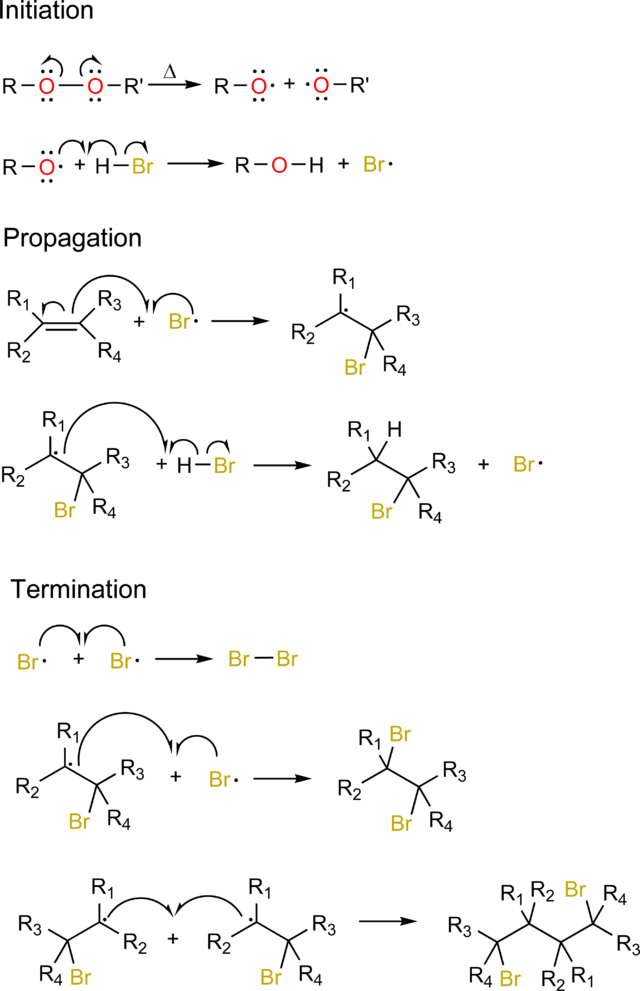
\includegraphics[width=0.7\textwidth]{img/roor}
    \label{fig.roor}
\end{figure}

\section{Ozonoliza}

Ozonolizę prowadzi się traktując badany alken ozonem $(O_3)$ a następnie redukuje się powstały produkt pośredni za pomocą cynku w środowisku jonu hydroniowego. Metoda ta znajduje zastosowanie w określaniu położenia wiązania podwójnego w cząsteczce.
\vspace{1cm}

\schemestart
    \chemfig{-[1]=[7]-[1]-[7]}
    \arrow{->[$O_3$][$Zn$,$H_3O^+$]}
    \chemfig{-[1]=[7]O}
    \+
    \chemfig{O=[7]-[1]-[7]}
\schemestop

\section{Dieny}

Dieny jest to grupa organicznych związków chemicznych, węglowodory nienasycone, w których występują dwa wiązania podwójne między atomami węgla.

W zależności od liczby wiązań pojedynczych znajdujących się pomiędzy wiązaniami podwójnymi w łańcuchu węglowym rozróżnia się trzy rodzaje dienów:

\subsection{Skumulowane}

Zwane są one allenami, w których wiązania podwójne sąsiadują ze sobą.
\vspace{0.5cm}

\chemfig{-[7]=[1]=[7]-[1]-[7]}

\subsection{Sprzężone}

Wiązania podwójne są w nich rozdzielone wiązaniem pojedynczym.
\vspace{0.5cm}

\chemfig{-[7]=[1]-[7]=[1]-[7]}

\subsection{Izolowane}

Pomiędzy wiązaniami podwójnymi występują conajmniej dwa wiązania pojedyncze.
\vspace{0.5cm}

\chemfig{-[7]=[1]-[7]-[1]=[7]}

\end{document}